%%%%%%%%%%%%%%%%%%%%%%%%%%%%%%%%%%%%%%%%%
%
% Space Physics
% Practical 2B
%
%%%%%%%%%%%%%%%%%%%%%%%%%%%%%%%%%%%%%%%%%

%----------------------------------------------------------------------------------------
%	DOCUMENT CONFIGURATIONS
%----------------------------------------------------------------------------------------

\documentclass{article}

\title{\textbf {Space Physics} \\ Practical 2B\\ Data Analysis} % Title
\def\authorivan{Ivan \v Sinkarenko}
\def\authoranu{Anuraj Rajendraprakash}
\author{\authorivan\\\authoranu}

\usepackage{graphicx}
\usepackage{fullpage}
\usepackage{url}
%\usepackage{color}

% load package with ``framed'' and ``numbered'' option.
\usepackage[framed,numbered,autolinebreaks,useliterate]{mcode}

\begin{document}

\maketitle % Insert the title, author and date

\centerline{Referee: Gabriella Stenberg}

\setlength\parindent{0pt} % Removes all indentation from paragraphs

\renewcommand{\labelenumi}{\alph{enumi}} % Make numbering in the enumerate environment by letter rather than number
\clearpage

\tableofcontents

\listoffigures

\clearpage

%----------------------------------------------------------------------------------------
%	SECTION 1. Introduction
%----------------------------------------------------------------------------------------
\section{Introduction}

    

%----------------------------------------------------------------------------------------
%	SECTION 2. Time Series Data
%----------------------------------------------------------------------------------------
\section{Time Series Data}

\subsection{Question 1}
\textit{Where in the magnetosphere are the observations made? Motivate you
answer!}

The measurment taken on 2002-03-02 at 03:29-03:30 is taken at the time when the satellite was crossing the border of magnetopause.

\begin{figure}[htb]
\centering
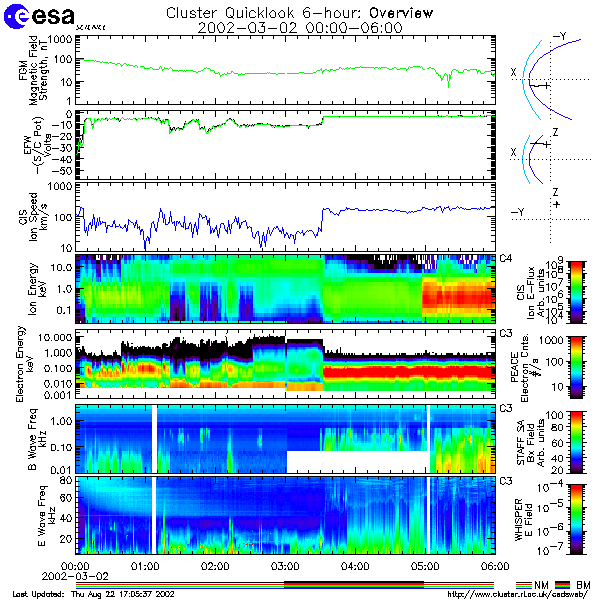
\includegraphics[width=0.7\textwidth]{Figures/cluster.png}
\caption{Cluster Quicklook 6-hours overview.}
\label{fig:cluster}
\end{figure}

\subsection{Question 2}
\textit{Plot the time series (all components) from the three instruments. Can you identify any waves? What type of waves are we looking at: Electrostatic or electromagnetic? Is there a need to correct the data somehow? If so, why and how do you do that?}

Electromagnetic between 20 and 30 s. Electrostatic between 55 and 60 s. x component is facing towards the sun. It should fluctuate around zero, like the y-component does it. It happens because of the photon emission, which is captured by the probes. Thus, data correction is needed.

\begin{figure}[htb]
\centering
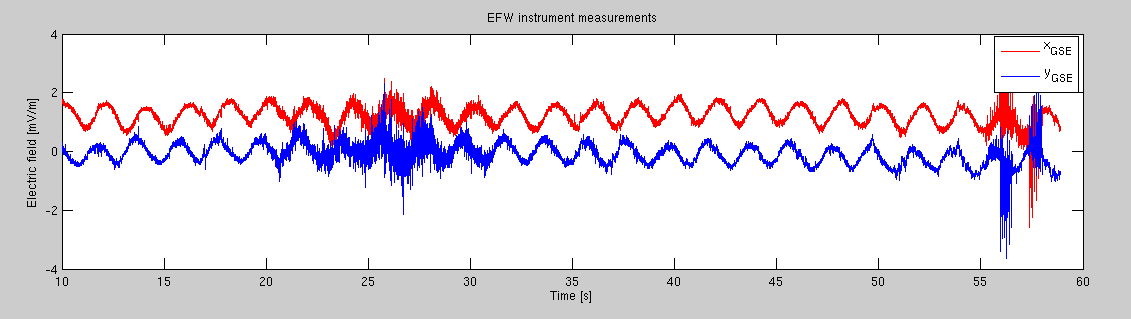
\includegraphics[width=\textwidth]{Figures/EFW_measurement.png}
\caption{EFW Measurement Data}
\label{fig:EFW}
\end{figure}

\begin{figure}[htb]
\centering
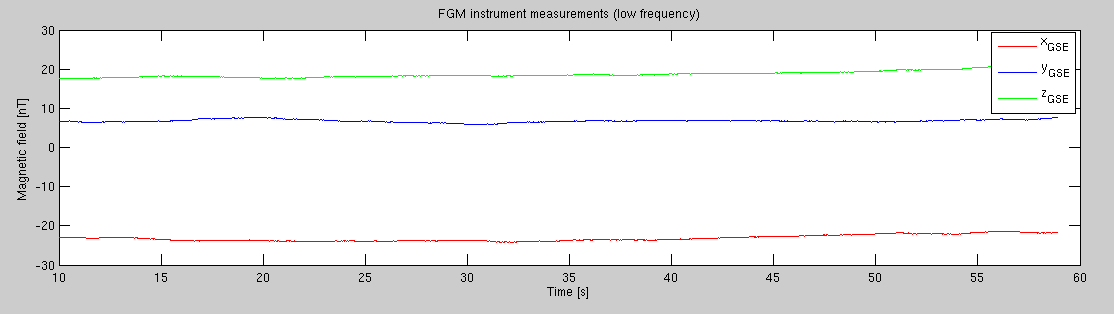
\includegraphics[width=\textwidth]{Figures/FGM_measurement.png}
\caption{FGM Measurement Data}
\label{fig:FGM}
\end{figure}

\begin{figure}[htb!]
\centering
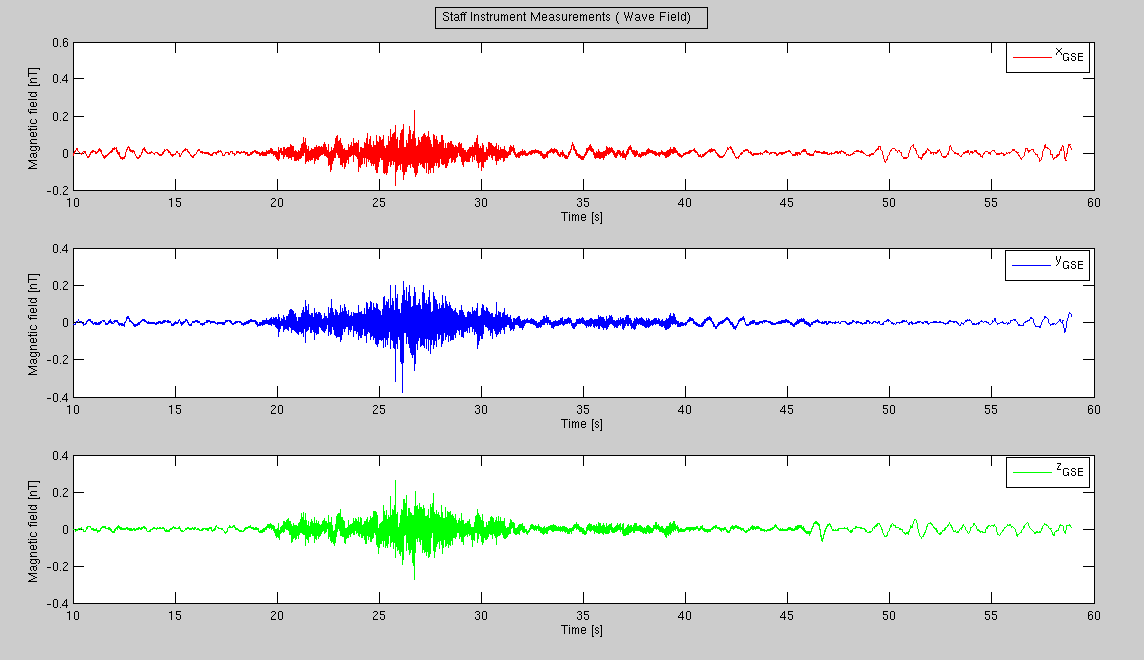
\includegraphics[width=\textwidth]{Figures/Staff_measurement.png}
\caption{Staff Instrument Measurement Data}
\label{fig:Staff}
\end{figure}

\subsection{Question 3}
\textit{Estimate the frequency of the waves by looking at the times series only. Describe how you do. What is you result?}

Roughly estimated wave period is about 0.01 s (zoomed in and estimated between 2 peaks). Frequency = 1/0.01 = 100 Hz.

\subsection{Question 4}
\textit{Compute the fundamental frequencies (electron and proton gyrofrequencies and the electron plasma frequency) in the plasma. The background magnetic field you have in the data. The density can be found from the overview data. However, the ion density is usually underestimated. Therefore, it is a good idea to compare with the high frequency emissions obtained by the WHISPER instrument. In the WHISPER data you can identify the electron plasma frequency directly, as a thin horizontal line visible most of the time. What density does the WHISPER signal correspond to? Compare the wave frequency with the fundamental frequencies. What are you conclusions?}

From overview data, ion density is $~1.5 cm^3$. 

The estimated plasma frequency from WHISPER is 16 kHz.

\subsection{Question 5}
\textit{Compute the PSD of the electric and magnetic wave fields for the entire time period. If you want you can use the Matlab-function PSDvsFREQ(). Compare with your results obtained in 2 and 3. Change the resolution of the PSD to clearly resolve the frequencies you found in 2. The frequency resolution is given by $Δf=1/NΔt$, where Δt is the time between two samples and N is the record length used in the Fourier transform.}

The peaks are around 90-100 Hz. Which corresponds to our rough estimation in question 3.

\begin{figure}[ht]
\begin{minipage}[c]{0.5\linewidth}
\centering
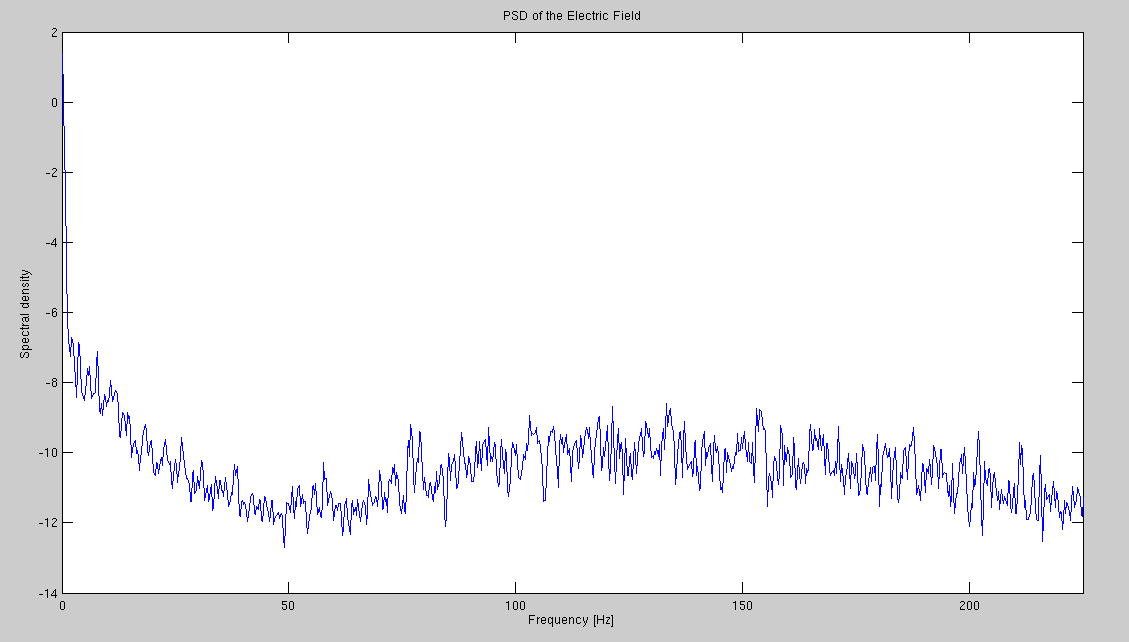
\includegraphics[width=8cm]{Figures/PSD_electric.png}
\caption{PSD of Electric Field.}
\label{fig:PSD_electric}
\end{minipage}
\hspace{0.1cm}
\begin{minipage}[c]{0.5\linewidth}
\centering
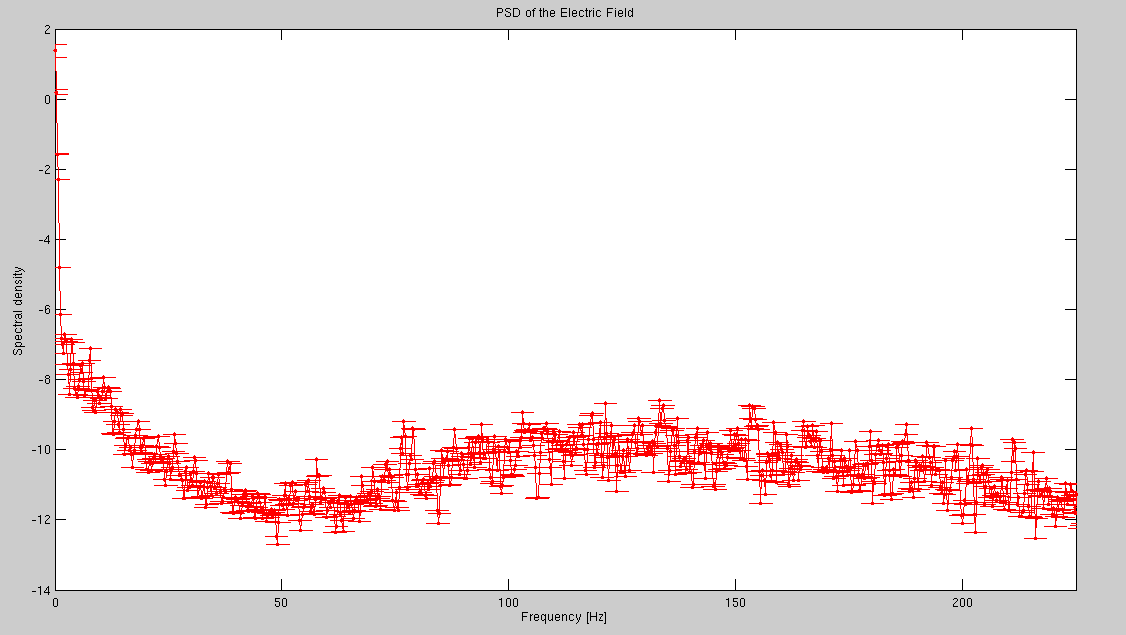
\includegraphics[width=8cm]{Figures/PSD_electric_error.png}
\caption{PSD of Electric Field with Error Bar}
\label{fig:PSD_electric_error}
\end{minipage}
\end{figure}

\begin{figure}[ht]
\begin{minipage}[c]{0.5\linewidth}
\centering
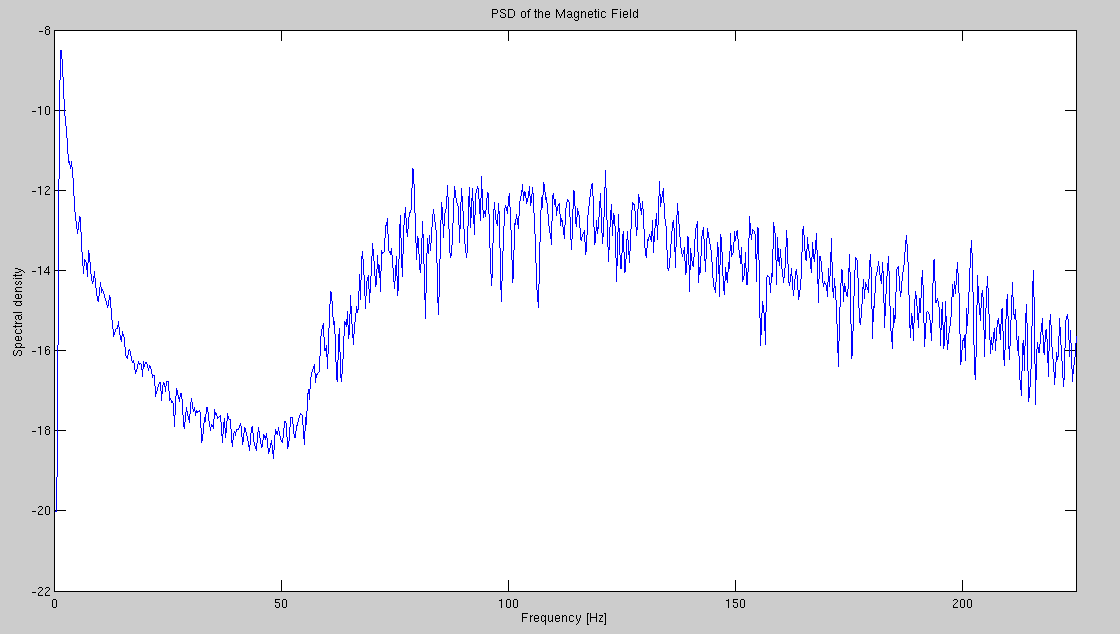
\includegraphics[width=8cm]{Figures/PSD_magnetic.png}
\caption{PSD of Magnetic Field.}
\label{fig:PSD_magnetic}
\end{minipage}
\hspace{0.1cm}
\begin{minipage}[c]{0.5\linewidth}
\centering
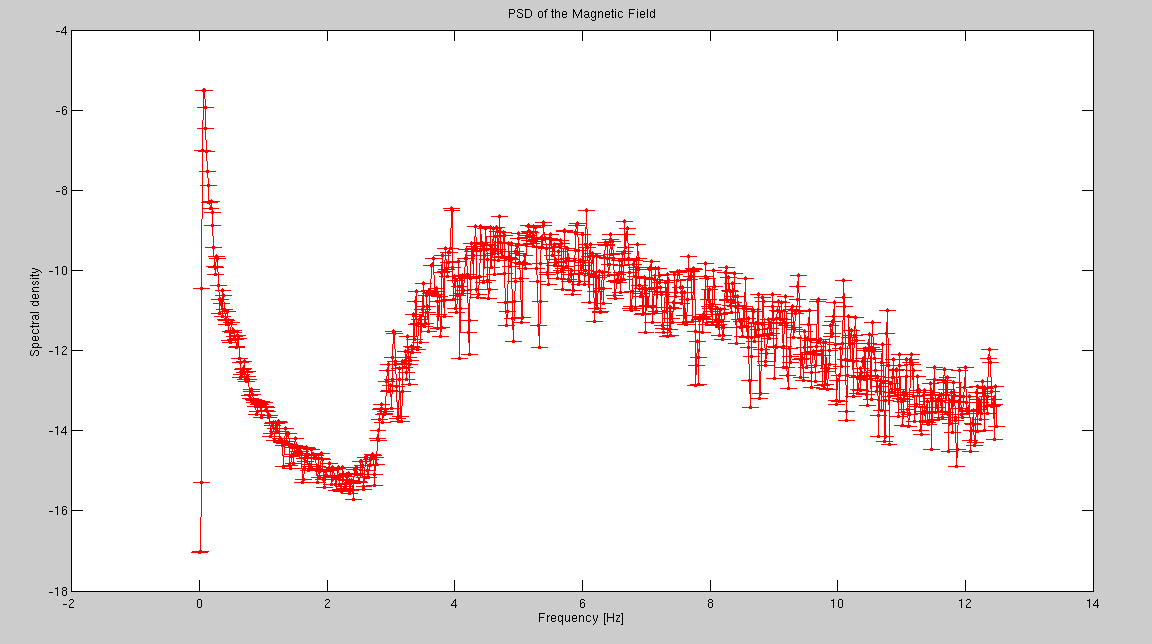
\includegraphics[width=8cm]{Figures/PSD_magnetic_error.png}
\caption{PSD with Error Bar}
\label{fig:PSD_magnetic_error}
\end{minipage}
\end{figure}

\begin{figure}[ht]
\begin{minipage}[c]{0.5\linewidth}
\centering
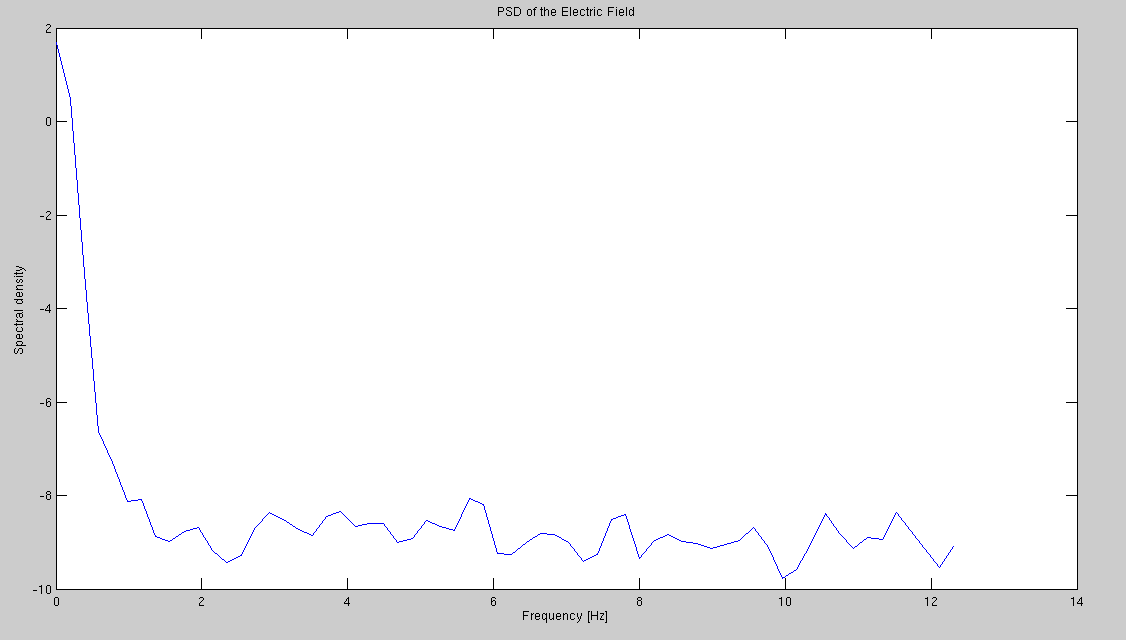
\includegraphics[width=8cm]{Figures/PSD_electric_L.png}
\caption{PSD of Electric Field with less records}
\label{fig:PSD_electric}
\end{minipage}
\hspace{0.1cm}
\begin{minipage}[c]{0.5\linewidth}
\centering
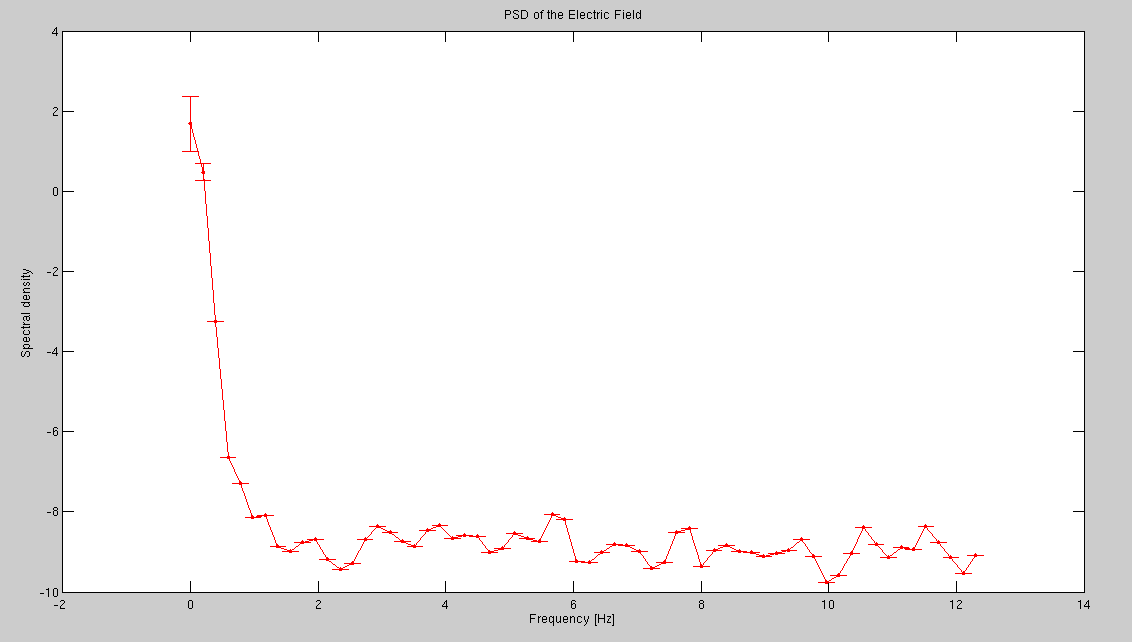
\includegraphics[width=8cm]{Figures/PSD_electric_errorL.png}
\caption{PSD with Error Bar and less records}
\label{fig:PSD_electric_error}
\end{minipage}
\end{figure}

\begin{figure}[ht]
\begin{minipage}[c]{0.5\linewidth}
\centering
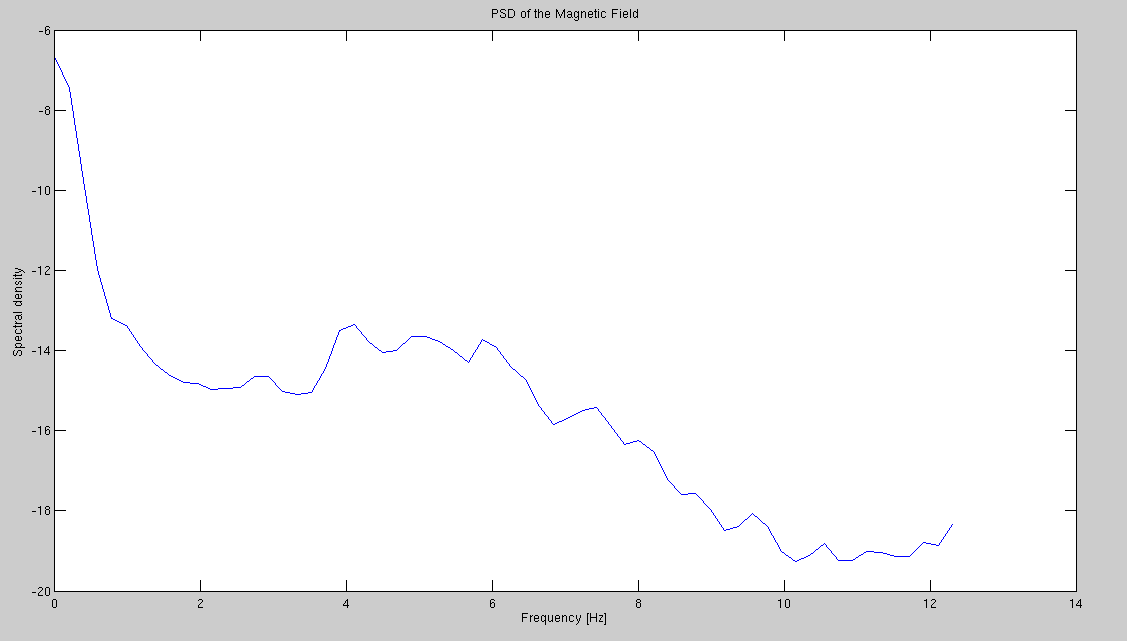
\includegraphics[width=8cm]{Figures/PSD_magnetic_L.png}
\caption{PSD of Magnetic Field with less records.}
\label{fig:PSD_magnetic}
\end{minipage}
\hspace{0.1cm}
\begin{minipage}[c]{0.5\linewidth}
\centering
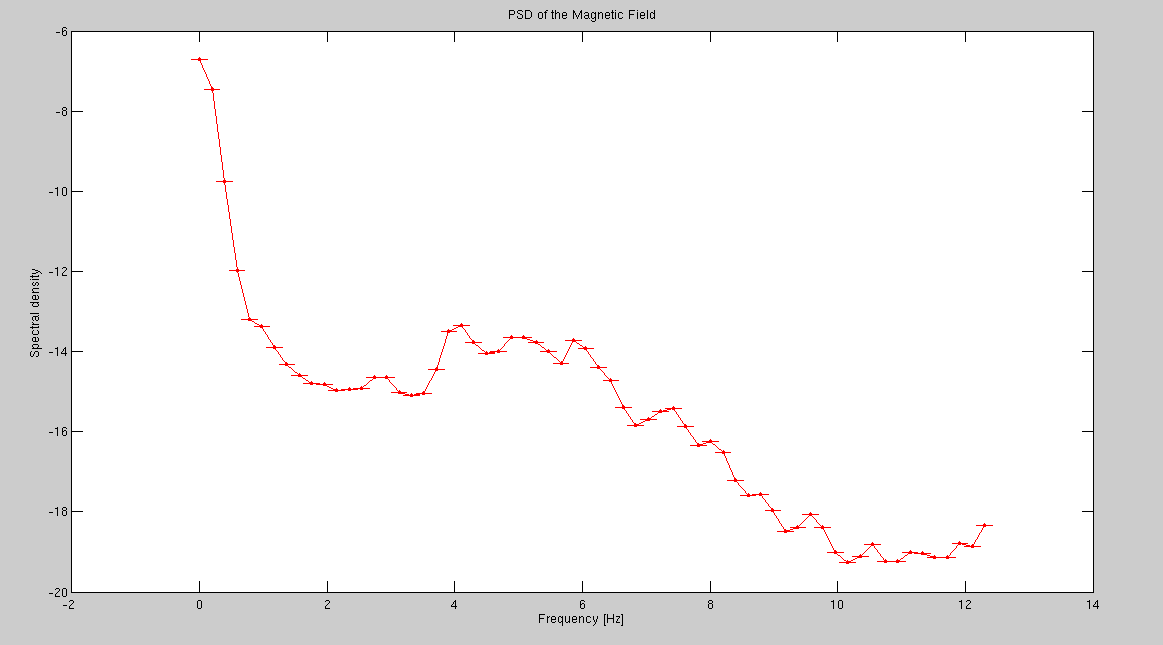
\includegraphics[width=8cm]{Figures/PSD_magnetic_errorL.png}
\caption{PSD with Error Bar with less records}
\label{fig:PSD_magnetic_error}
\end{minipage}
\end{figure}


\subsection{Question 6}
\textit{Look at (=make PSDs for) two different frequency ranges: 0-225 Hz and 0-2 Hz. You should aim at good statistics so the frequency resolution should be different in the two plots. The frequency resolution is given by $Δf=1/NΔt$, where Δt is the time between two samples and N is the record length used in the Fourier transform. For each of the plots: provide all the information about the PSD you present: The length of the record, the shift between records and the total number of records used.}

\subsection{Question 7}
\textit{Plot spectrograms (=PSD versus time and frequency) of both the electric and magnetic fields. You can do this by using the Matlab function means() and ignoring the wave vector output. Try different resolutions in time and frequency.What are you conclusions?}

\begin{figure}[ht]
\begin{minipage}[c]{0.5\linewidth}
\centering
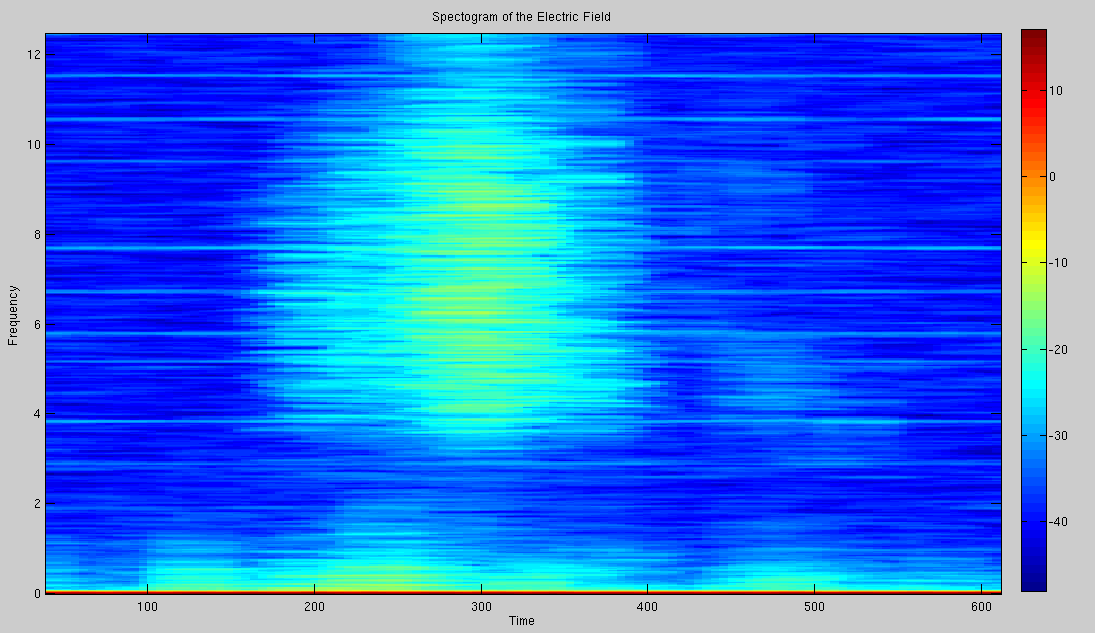
\includegraphics[width=8cm]{Figures/spectrogram_electricHR.png}
\caption{Spectrogram of Electric Field with high time and frequency resolution}
\label{fig:spectrogram_electricHR}
\end{minipage}
\hspace{0.1cm}
\begin{minipage}[c]{0.5\linewidth}
\centering
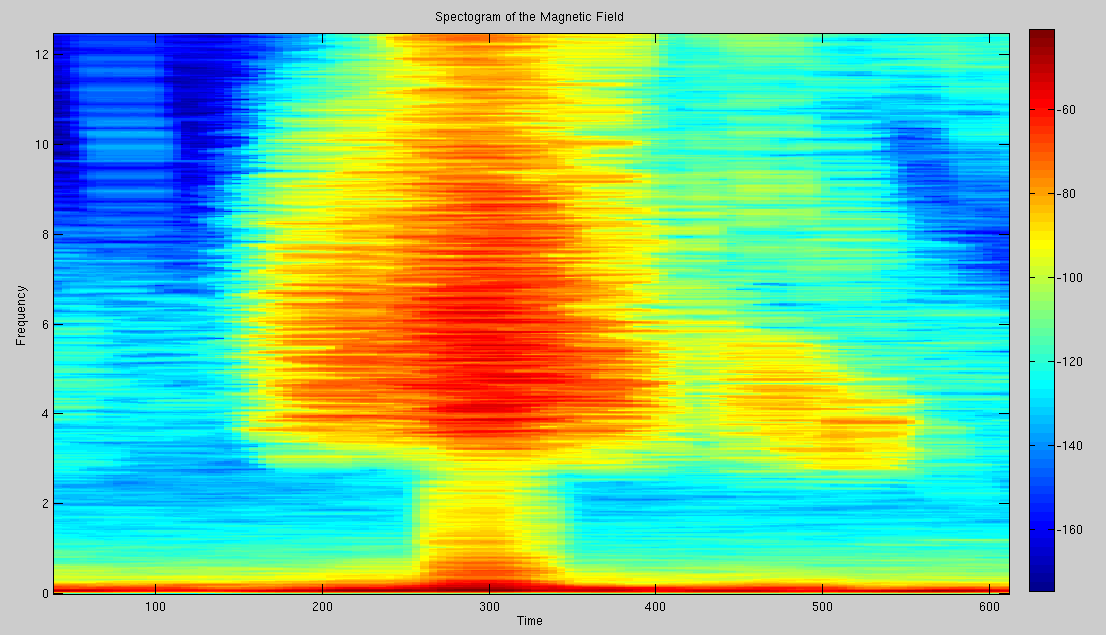
\includegraphics[width=8cm]{Figures/spectrogram_magneticHR.png}
\caption{Spectrogram of Magnetic Field with high time and frequency resolution}
\label{fig:spectrogram_magneticHR}
\end{minipage}
\end{figure}

\begin{figure}[ht]
\begin{minipage}[c]{0.5\linewidth}
\centering
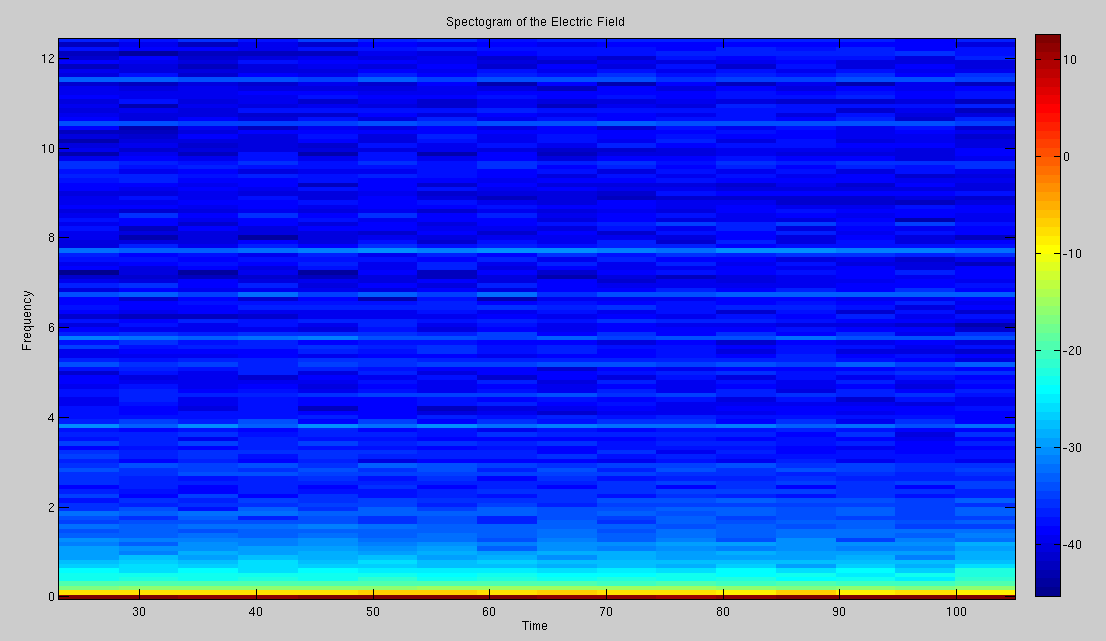
\includegraphics[width=8cm]{Figures/spectrogram_electricLR.png}
\caption{Spectrogram of Electric Field with low time and frequency resolution}
\label{fig:spectrogram_electricLR}
\end{minipage}
\hspace{0.1cm}
\begin{minipage}[c]{0.5\linewidth}
\centering
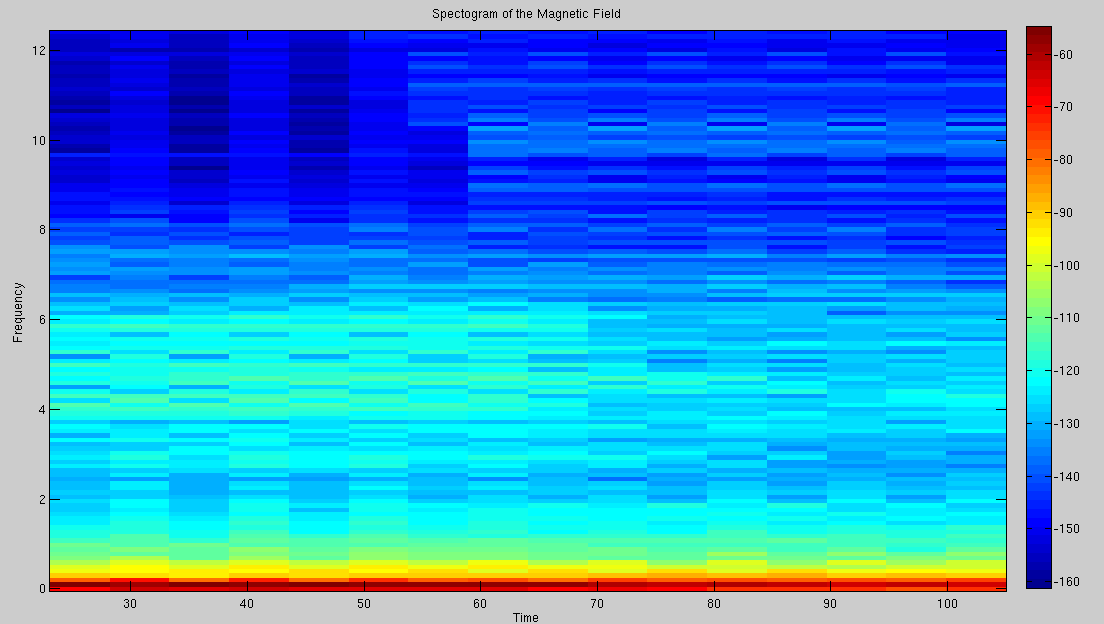
\includegraphics[width=8cm]{Figures/spectrogram_magneticLR.png}
\caption{Spectrogram of Magnetic Field with low time and frequency resolution}
\label{fig:spectrogram_magneticLR}
\end{minipage}
\end{figure}

\subsection{Question 7}
\textit{Now we can produce a so-called hodogram , which shows how the wave field vector moves in the plane perpendicular to B0. If the field vector moves in the same direction as a positive ion would gyrate then the wave is left-hand polarized. If the vector rotates in the opposite direction the wave is righthand polarized. Plot the magnetic field vector in this plane and determine the polarization of the waves. Sometimes it is easier to see the rotation if you normalize the length of the vectors to 1. Do the same with the electric field wave vector.}

\clearpage
%----------------------------------------------------------------------------------------
%	SECTION 2. PARTICLE MEASUREMENTS
%----------------------------------------------------------------------------------------
\section{Particle Measurements}

For this part of the practical we have been provided the particle data from the SWIM
instrument onboard the Chandrayaan-1 spacecraft. Chandrayaan-1 orbits the moon at an altitude of 100 km. The position of the spacecraft at different times is shown in the Figures \ref{fig:orbit_1069} and \ref{fig:orbit_1070}, which also show the position of the moon with respect to Earth.

\begin{figure}[ht]
\begin{minipage}[c]{0.5\linewidth}
\centering
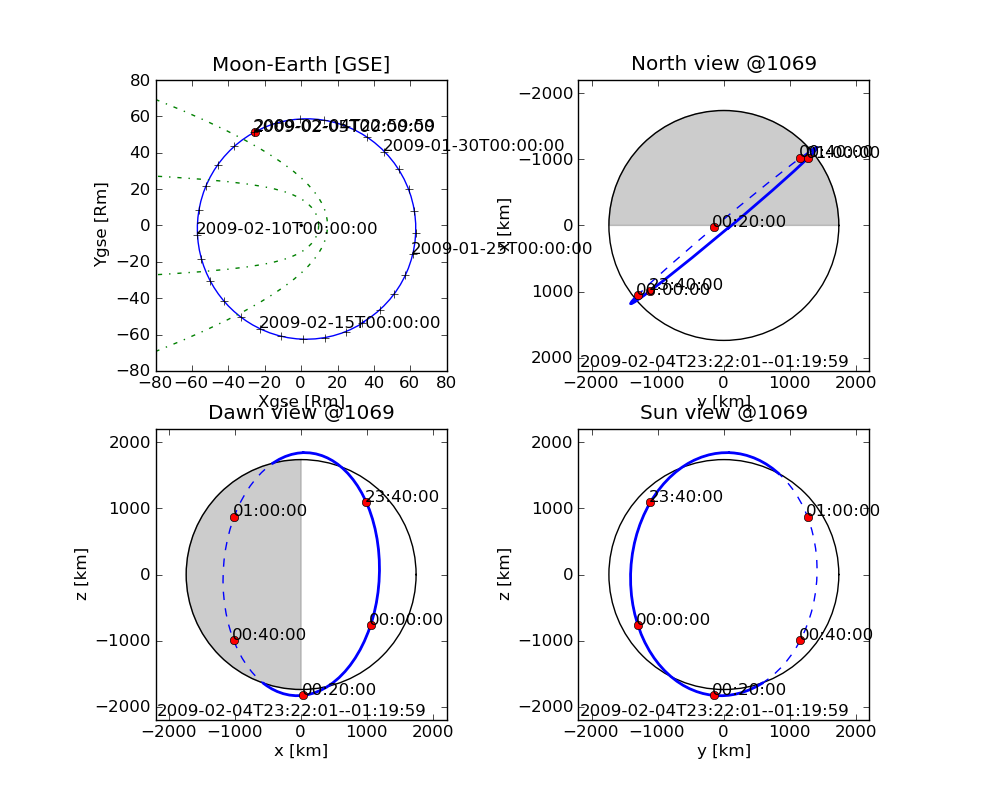
\includegraphics[width=9cm]{Figures/orbit_1069.png}
\caption{Position of the instrument in Orbit 1069}
\label{fig:orbit_1069}
\end{minipage}
\hspace{0.2cm}
\begin{minipage}[c]{0.5\linewidth}
\centering
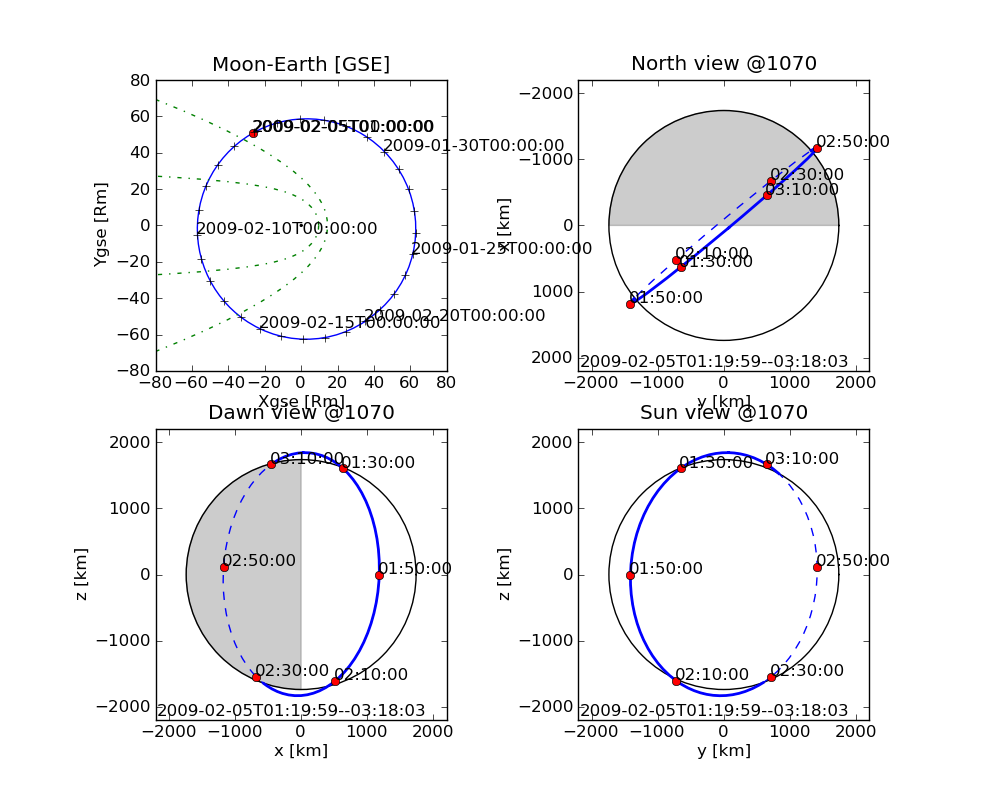
\includegraphics[width=9cm]{Figures/orbit_1070.png}
\caption{Position of the instrument in Orbit 1070}
\label{fig:orbit_1070}
\end{minipage}
\end{figure}


\subsection{Question 1}
\textit{Plot spectrograms, that is, the number of counts versus time and energy, for the
two orbits. The different energy levels you find in a comment line in the data files.
Once every orbit SWIM looks at the solar wind. Identify when this happens in the two
orbits.}

The spectrograms for the orbits 1069 and 1070 is shown in Figure \ref{fig:spectrogram_1069} and \ref{fig:spectrogram_1070} respectively. When SWIM looks at the solar wind the number of solar wind particles that hit the instrument increases significantly which is observable as the red portion in Figures \ref{fig:spectrogram_1069} and \ref{fig:spectrogram_1070}. For orbit 1069, it occurs approximately between $100th$ and $350th$ observation time bin which corresponds to UTC 05:29 to UTC 06:02 hours. For orbit 1070, it occurs approximately between $25th$ and $250th$ observation time bin which corresponds to UTC 07:22 to UTC 08:12 hours.

\begin{figure}[h!]
\centering
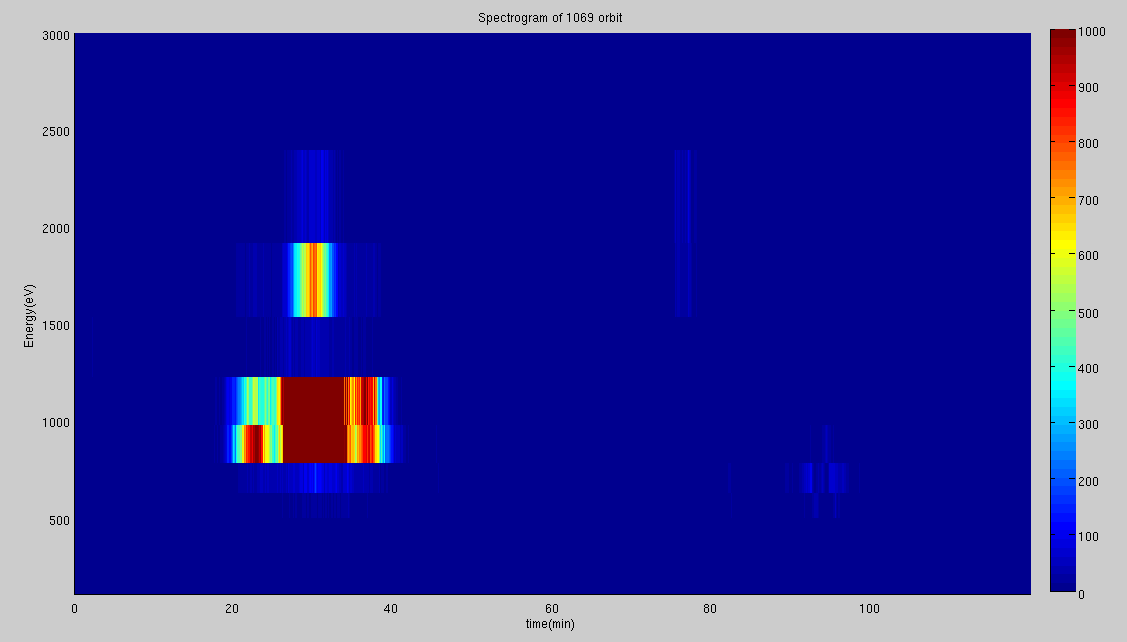
\includegraphics[scale=0.35]{Figures/spectrogram_1069.png}
\caption{Spectrogram of the 1069 Orbit}
\label{fig:spectrogram_1069}
\end{figure}

\begin{figure}[h!]
\centering
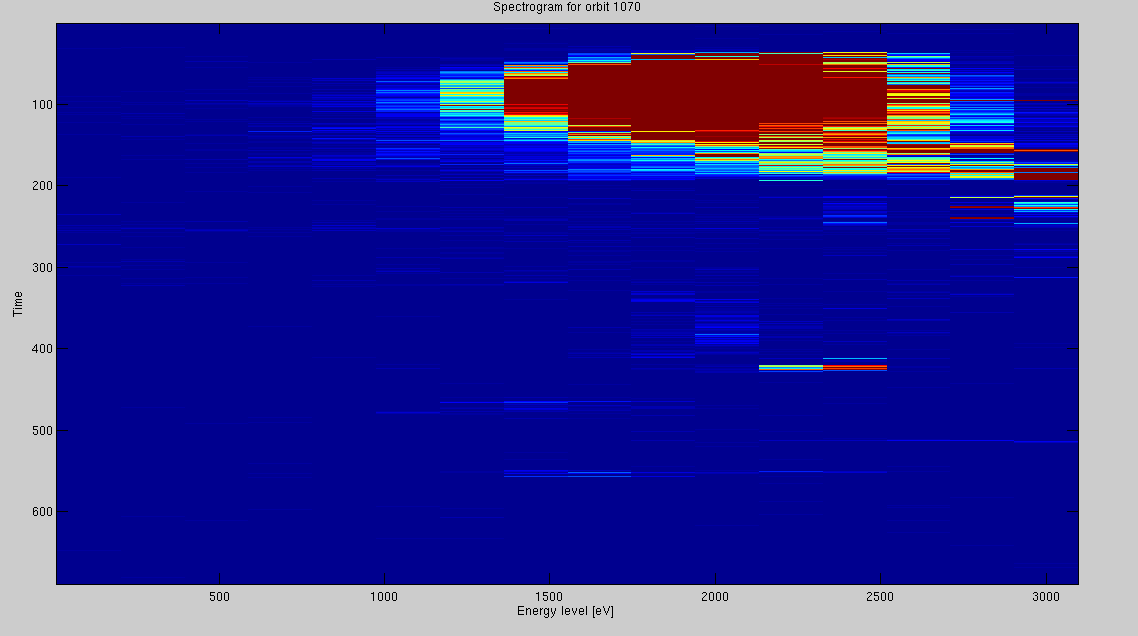
\includegraphics[scale=0.35]{Figures/spectrogram_1070.png}
\caption{Spectrogram of the 1070 Orbit}
\label{fig:spectrogram_1070}
\end{figure}

\subsection{Question 2}
\textit{Protons are the main ions in the solar wind, but can you identify any other
components? Motivate you answer!}

{\color{red} Helium double plus. I am not sure.}

\subsection{Question 3}
\textit{Make energy spectra, this is, plot observed counts versus energy for a selected
time interval around the solar wind observation.}

The energy spectra for the time when the SWIM instrument looks at the solar wind for the orbit 1069 and orbit 1070 is shown in Figure \ref{fig:energy_spectra_1069} and \ref{fig:energy_spectra_1070} respectively

\begin{figure}[h!]
\centering
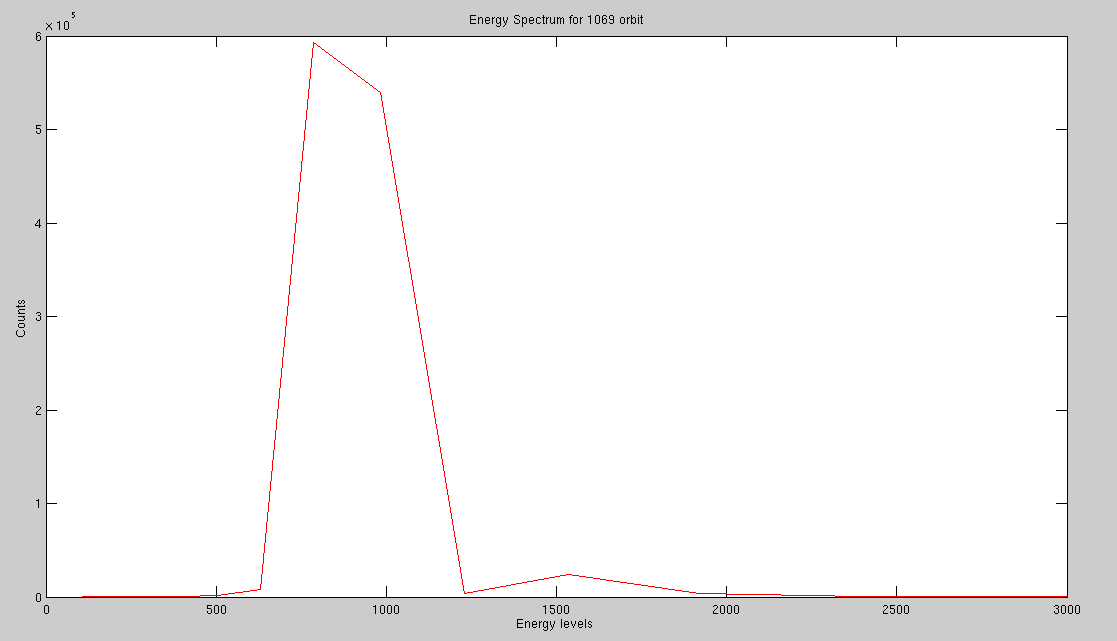
\includegraphics[scale = 0.35]{Figures/energy_spectra_1069.png}
\caption{Energy Spectra of the 1069 Orbit}
\label{fig:energy_spectra_1069}
\end{figure}

\begin{figure}[h!]
\centering
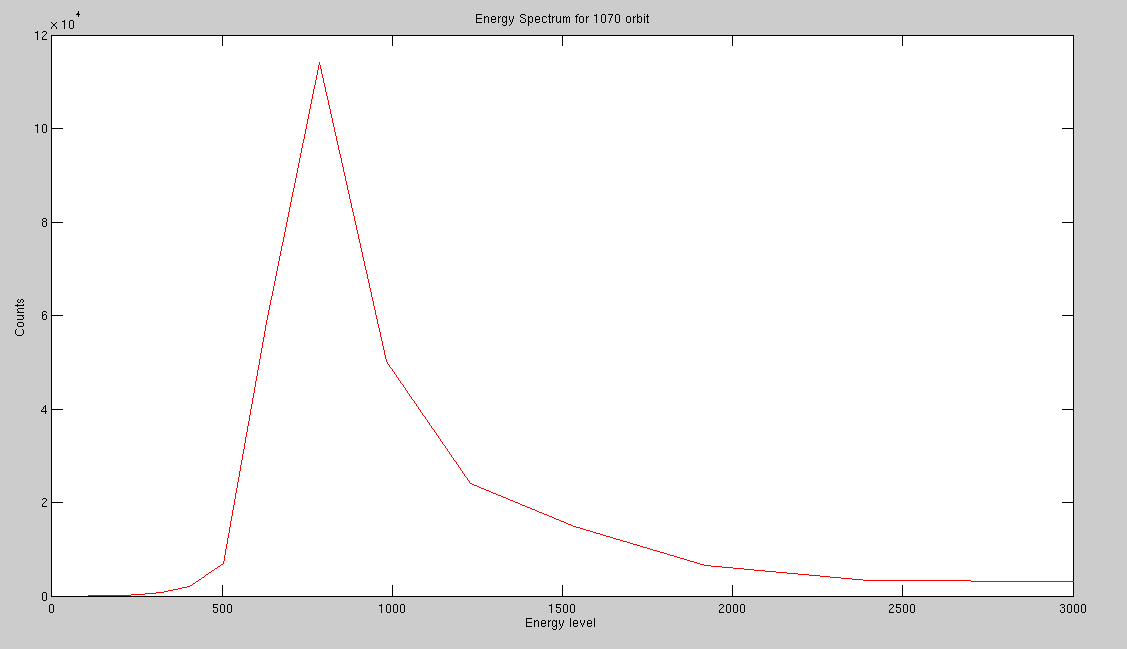
\includegraphics[scale = 0.35]{Figures/energy_spectra_1070.png}
\caption{Energy Spectra of the 1070 Orbit}
\label{fig:energy_spectra_1070}
\end{figure}

\subsection{Question 4}
\textit{Determine the solar wind proton velocity and temperature by first transforming the
data from energy to velocity space and then fitting a Maxwellian distribution. What
temperatures and velocities do you get? Are there differences between the orbits? If
so, why?}

\begin{figure}[!ht]
\centering
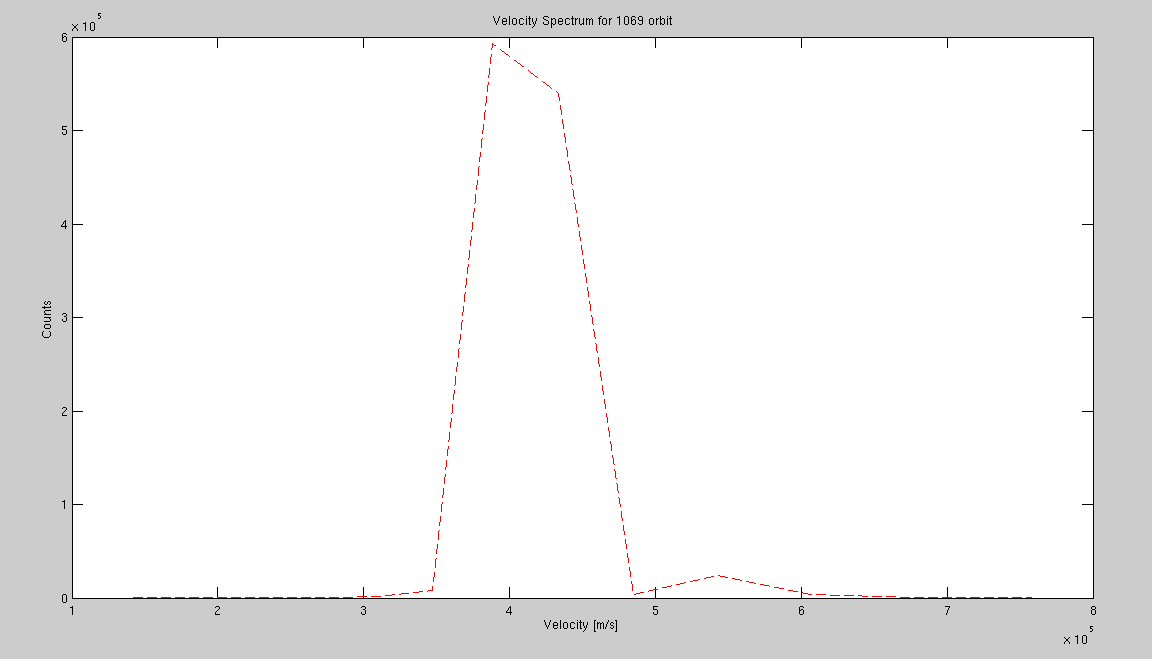
\includegraphics[scale=0.35]{Figures/velocity_spectra_1069.png}
\caption{Velocity Spectra of the 1069 Orbit}
\label{fig:Velocity_spectra_1069}
\end{figure}

\begin{figure}
\centering
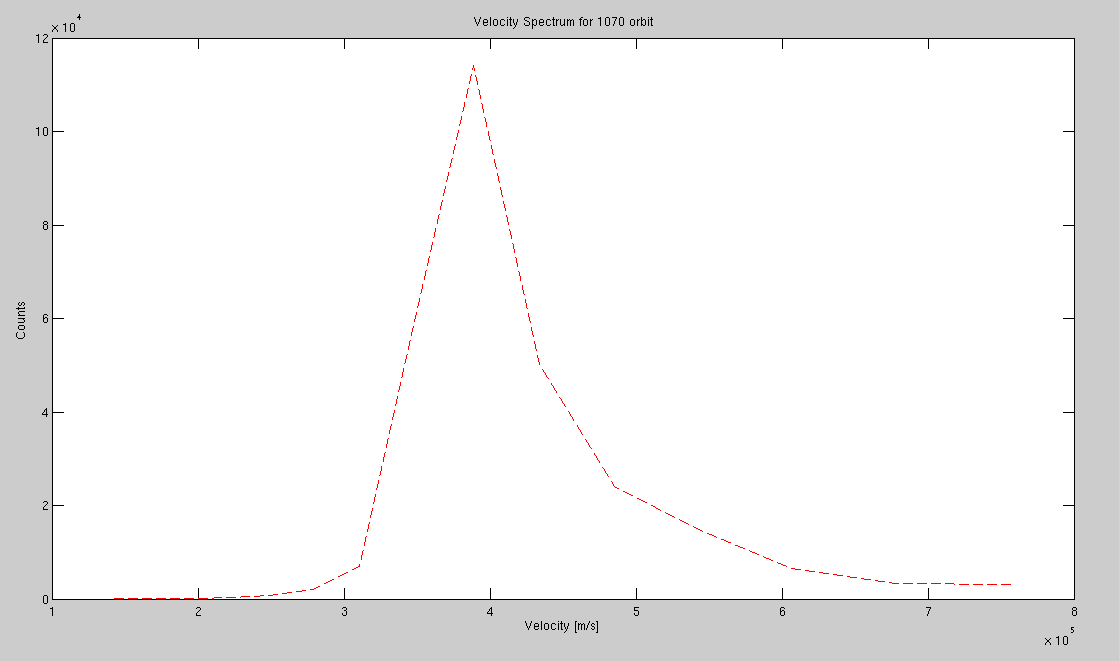
\includegraphics[scale=0.35]{Figures/velocity_spectra_1070.png}
\caption{Velocity Spectra of the 1070 Orbit}
\label{fig:Velocity_spectra_1070}
\end{figure}

\begin{figure}[!ht]
\centering
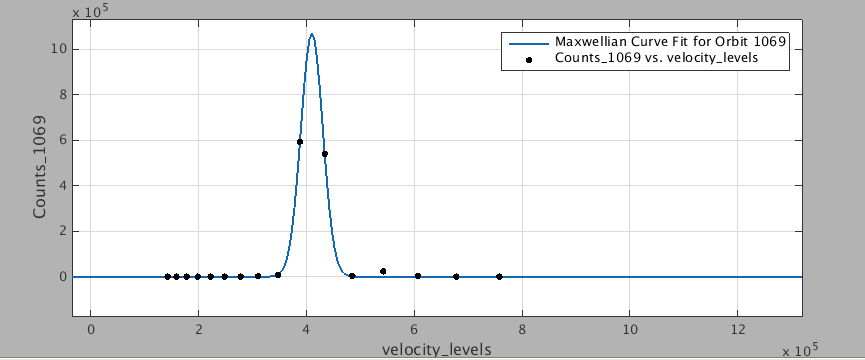
\includegraphics[scale=0.45]{Figures/curvefit_1069.png}
\caption{Maxwellian Curve fit for data from Orbit 1069}
\label{fig:curvefit_1069}
\end{figure}

\begin{figure}
\centering
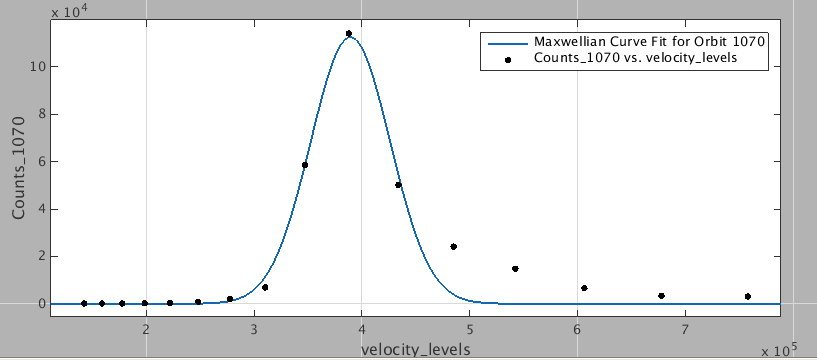
\includegraphics[scale= 0.45]{Figures/curvefit_1070.png}
\caption{Maxwellian Curve fit for data from Orbit 1070}
\label{fig:curvefit_1070}
\end{figure}


%----------------------------------------------------------------------------------------
%	SECTION 3. CONCLUSION
%----------------------------------------------------------------------------------------
%\newpage
\section{Conclusion}



%----------------------------------------------------------------------------------------
%	SECTION 4. REFERENCES
%----------------------------------------------------------------------------------------
\newpage
\begin{thebibliography}{9}

\bibitem{Enmark:2012a3}
Enmark A.  (2012).
\newblock {\em Assignment 3. Optimization of phased array antenna radiation pattern and array configuration}.
\newblock Lule\aa \ University of Technology, Kiruna, Sweden.

\bibitem{Skolnik:2001irs}
Skolnik M. ~I.  (2001).
\newblock {\em Introduction to Radar Systems}.
\newblock The McGraw-Hill Companies, Inc., New York, United States.

\bibitem{Rottger:2000ip}
R\"ottger J.  (2000).
\newblock {\em The Instrumental Principles of MST Radars and Incoherent Scatter Radars and The Configuration of Radar System Hardware}.
\newblock Max Planck Institut F\"ur Aeronomie, Katlenburg-Lindau, Germany.

\bibitem{Wiki:2012pa}
Wikipedia.org. (2012).
\newblock {\em Phased array}.
\newblock {\url{http://en.wikipedia.org/wiki/Phased_array}}.

\end{thebibliography}


%----------------------------------------------------------------------------------------
%	SECTION 5. Appendix 1
%----------------------------------------------------------------------------------------
\newpage
\section{Appendix 1. Matlab code}
%\lstinputlisting{assignment.m}

\end{document}